\documentclass[letter]{bioinfo}
\copyrightyear{2018} \pubyear{2018}

\access{Advance Access Publication Date: Day Month Year}
\appnotes{Review article}
\graphicspath{{../figures/}}

\newcommand{\comment}[1]{\textcolor{red}{#1}}
\newcommand{\todo}[1]{\colorbox{yellow}{\parbox{1\linewidth}{#1}}}

\begin{document}
\firstpage{1}

\subtitle{Review}

\title[short Title]{Cardioinformatics: the unmet need to pioneer an emerging field at the nexus of bioinformatics and cardiology}
\author[Sample \textit{et~al}.]{Bohdan B. Khomtchouk\,$^{\text{\sfb 1,}*}$, Diem-Trang Tran\,$^{\text{\sfb 2}}$, Themistocles L. Assimes\,$^{\text{\sfb 3, 4}}$ and Or Gozani\,$^{\text{\sfb 1}}$}
\address{$^{\text{\sf 1}}$Department of Biology, Stanford University, Stanford, CA, USA \\
$^{\text{\sf 2}}$School of Computing, University of Utah, Salt Lake City, UT, USA \\
$^{\text{\sf 3}}$Department of Medicine, Division of Cardiovascular Medicine, Stanford University, Stanford, CA, USA \\
$^{\text{\sf 4}}$VA Palo Alto Health Care System, Palo Alto, CA, USA
}

\corresp{$^\ast$To whom correspondence should be addressed.}

\history{Received on XXXXX; revised on XXXXX; accepted on XXXXX}

\editor{Associate Editor: XXXXXXX}

\abstract{\textbf{Motivation:} Text Text Text Text Text Text Text Text Text Text Text Text Text
Text Text Text Text Text Text Text Text Text Text Text Text Text Text Text Text Text Text Text
Text Text Text Text Text Text Text Text Text Text Text Text Text Text Text Text Text Text Text
Text Text Text Text Text Text
Text Text Text Text Text.\\
\textbf{Results:} Text  Text Text Text Text Text Text Text Text Text  Text Text Text Text Text
Text Text Text Text Text Text Text Text Text Text Text Text Text  Text Text Text Text Text Text\\
\textbf{Availability:} Text  Text Text Text Text Text Text Text Text Text  Text Text Text Text
Text Text Text Text Text Text Text Text Text Text Text Text Text Text  Text\\
\textbf{Contact:} \href{bohdan@stanford.edu}{bohdan@stanford.edu}\\
\textbf{Supplementary information:} Supplementary data are available at \textit{Briefings in Bioinformatics}
online.}

\maketitle

\section{The current status of bioinformatics in cardiovascular  research}
\begin{figure}
	\centering
	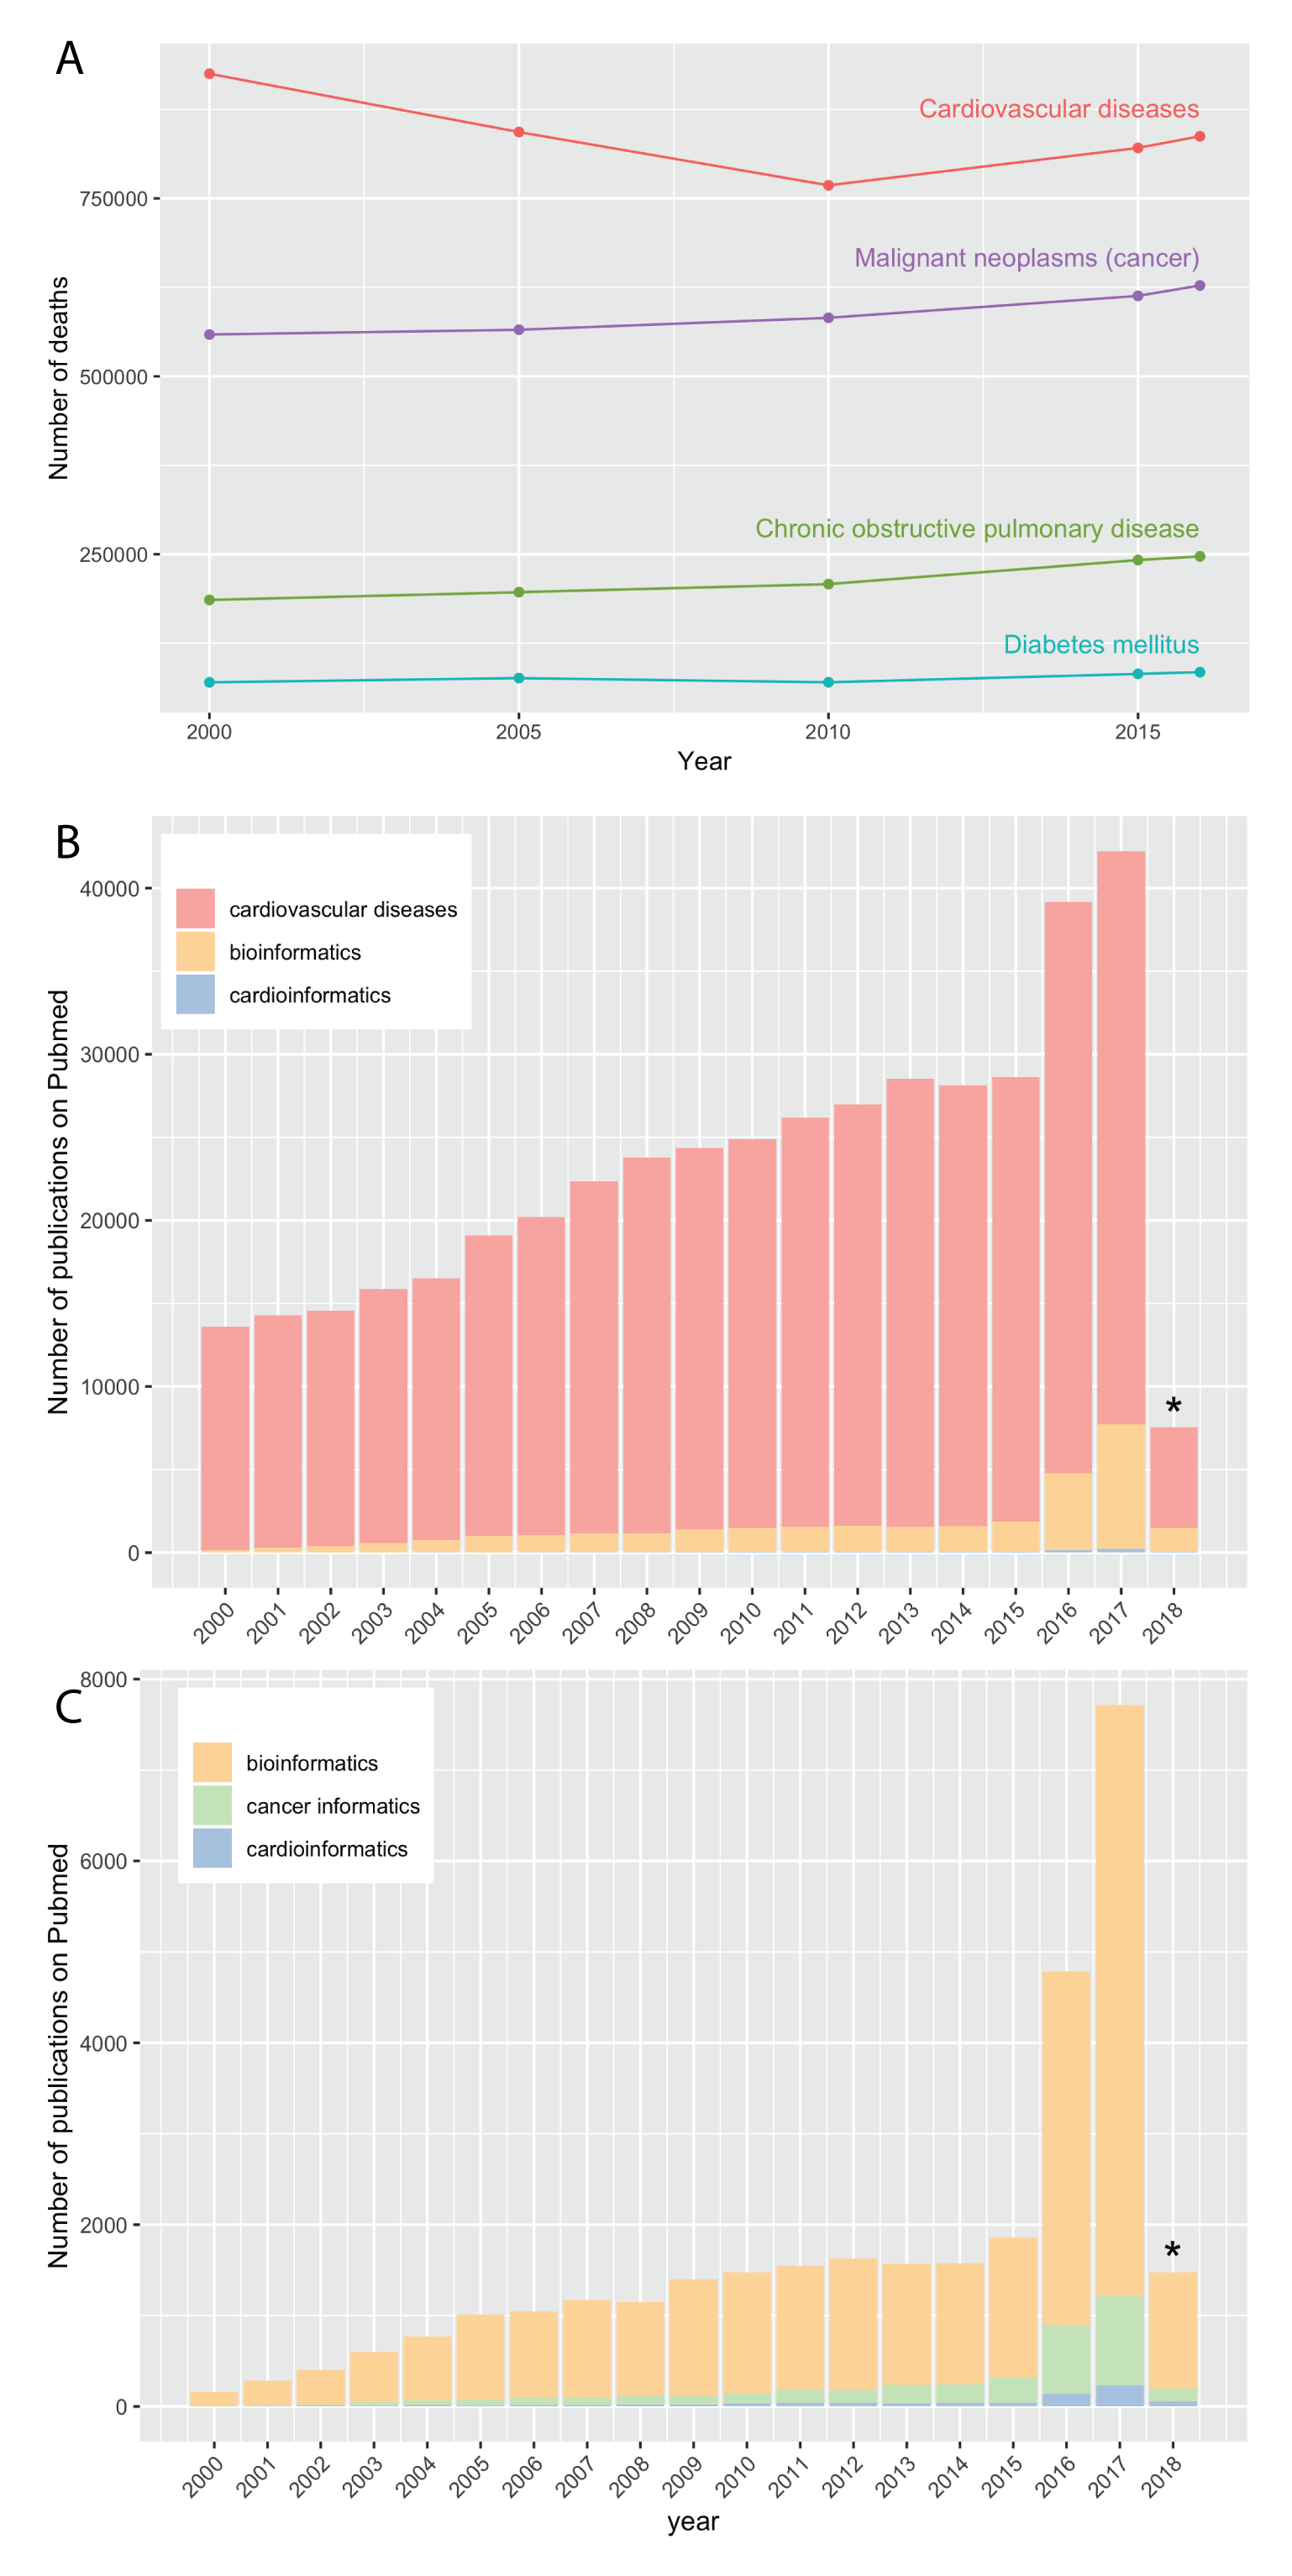
\includegraphics[width=1\linewidth]{figure1}
	\caption{\textbf{A}. Number of deaths by Non-Communicable Diseases in the US. \textbf{B}. \textbf{C}.}
	\label{fig:figure1}
\end{figure}

Cardiovascular diseases (CVD) have persistently been the leading cause of deaths by non-communicable diseases in the US for the last two decades (Figure \ref{fig:figure1}A). Research in CVD has steadily increased since 2000, as measured by the body of publications indexed in PubMed over the time (Figure \ref{fig:figure1}B). In 2017 alone, there are more than 40000 non-review articles classified with the subject heading "cardiovascular disease" (defined according to the Medical Subject Heading -- MeSH terms. The MeSH Database entry for \textit{cardiovascular disease} includes many types of cardiovascular abnormalities which may occur in organs other than the circulatory system.)

Among these outputs, the share of bioinformatics research remains modest, almost invisible. Despite the being present in the current tide of precision medicine initiatives, cardiovascular research is critically lacking in bioinformatics research which is at the center of precision medicine \citep{Gomez-Lopez:2017:Precision}.  The modest contribution of bioinformatics in cardiology is in stark contrast to that in cancer, to some extent suggesting that there are ample opportunities for cardioinformatics. Despite being "complex diseases". In this review, we highlight the contemporary problems in the research of CVD genetics, introduce the bountiful resources available and propose the ways to advance this field and leverage cardiovascular research with bioinformatics.

The first draft of the human genome project had brought a lot of hope and excitement about potential advancements in the diagnosis and treatment of cardiac diseases, such as the ability to identify disease genes within the associated loci, to improve risk estimation based on more precise genotypes, or to personalize the prediction of drug effect on a patient, \citep{Komajda:2001:heart}.


Outstanding problems

Variant calling and pathogenicity prediction. Currently inconsistent. Mostly developed for protein-coding fraction of the genome (SIFT, Polyphen, etc.), largely ignore the non-coding regions.
Pathogenicity assignment: variable, conflicting, not applicable for all populations.

Risk estimation

Lack of mechanistic understanding

Lack of platforms for accessible data and knowledge base

AHA precision medicine platform mark the presence of this field in precision medicine. However, the platform also exposed some critical issues \comment{Trang: re-visit AHA PMP for more specific points}. Unless we recognize the opportunities and tend to the challenges, cardiovascular research won't benefit from this new wave of methodological advance.


%{https://www.ncbi.nlm.nih.gov/mesh/68002318} 

As we further our quest to understand the genetics of heart diseases, many conditions have become too complicated for traditional approaches. Reflecting on the current body of knowledge, we recognize that many aspects of this complexity can be addressed with more computational methods.

\section{Complexity of CVDs}  % the problems

\subsection{The number of actors}

% large number --> small effects
% large number --> more interactions, intra and inter-pathways
% 
There are a certain genetic component in all major categories of heart diseases (Figure \ref{fig:hpo_gene_count}). As more studies are published, the number of genes found associated with a disease has also increased and in most cases, gone beyond a few genes that could be described in a single-page table or diagram.

As the most common cause of heart transplantation, dilated cardiomyopathy (DCM) worths investigating. In a recent review \citep{Burke:2016:Clinical} 16 disease-causing genes were compiled, along with an additional 41 putative genes. Meanwhile, GWAS catalog and HPO annotation suggested a much larger number of genes associated with this condition, 69 genes and 115 genes, respectively. Clinical application is keeping up, with a typical commercial gene panel for DCM genetic testing cover 50 genes on average, and 111 in total \citep{McNallyElizabethM.:2017:Dilated}.
%These numbers clearly advocate for more bioinformatics analyses to gain insights into this condition and the other conditions that are equivalently complex.
It is reasonably expected that when more genes are involved in a disease, the effect exerted by each gene gets smaller \comment{cite?}. Finding the significant associations of such small effect requires a much larger number of samples for sufficient power, or critically different methods of statistical testing and inference.\comment{Check refs. Elaborate on current efforts to have large study populations and to devise new way to fish for those associations.}

Beside the increasing difficulty discovering these genes, modeling of their effects is speedily complicated. With a potential interaction between every pair of genomic features, be they genes or regulatory sequences, the number of such interactions increase quadratically with the number of actors, leading to the combinatorial explosion of states that a biological system can assume.
Moreover, genetic interactions do not limit to those within a single biological pathway. Independent research in aging has unraveled the intertwined relation between heart disease and longevity pathways \citep{North:2012:Intersection}.  With age being the most important factor in constituting cardiovascular risk, it is unavoidable that an even larger number of genes and pathways will be involved in future analyses of CVD genetics.


does it help to have too many variants in a genetic risk score?

non-additive effects


%As with other complex diseases, missing heritability has been a long-standing puzzle in cardiovascular diseases \citep{Manolio:2009:Finding}. Despite the early successes in pinpointing the causes of several monogenic diseases, the large body of genome-wide association (GWA) studies have defied many widely held beliefs about genetic variants in human, hinting at the directions to search for the missing heritability.


%rare variants. The most trivial situation where inherited risk is not fully accounted for is when the variants are simply too rare to be detected with sufficient power. One addresses this issue by collecting more samples or improving statistical tests. \comment{This reason has driven a lot of efforts to enlarge and diversify the study population, but I can't seem to get the relation RARE => PATHOGENIC.} The availability of a large number of genomes and exomes, on one hand enabled the detection of such rare variants, and on the others,  showed that rare variants 


\begin{figure*}[!tpb]
	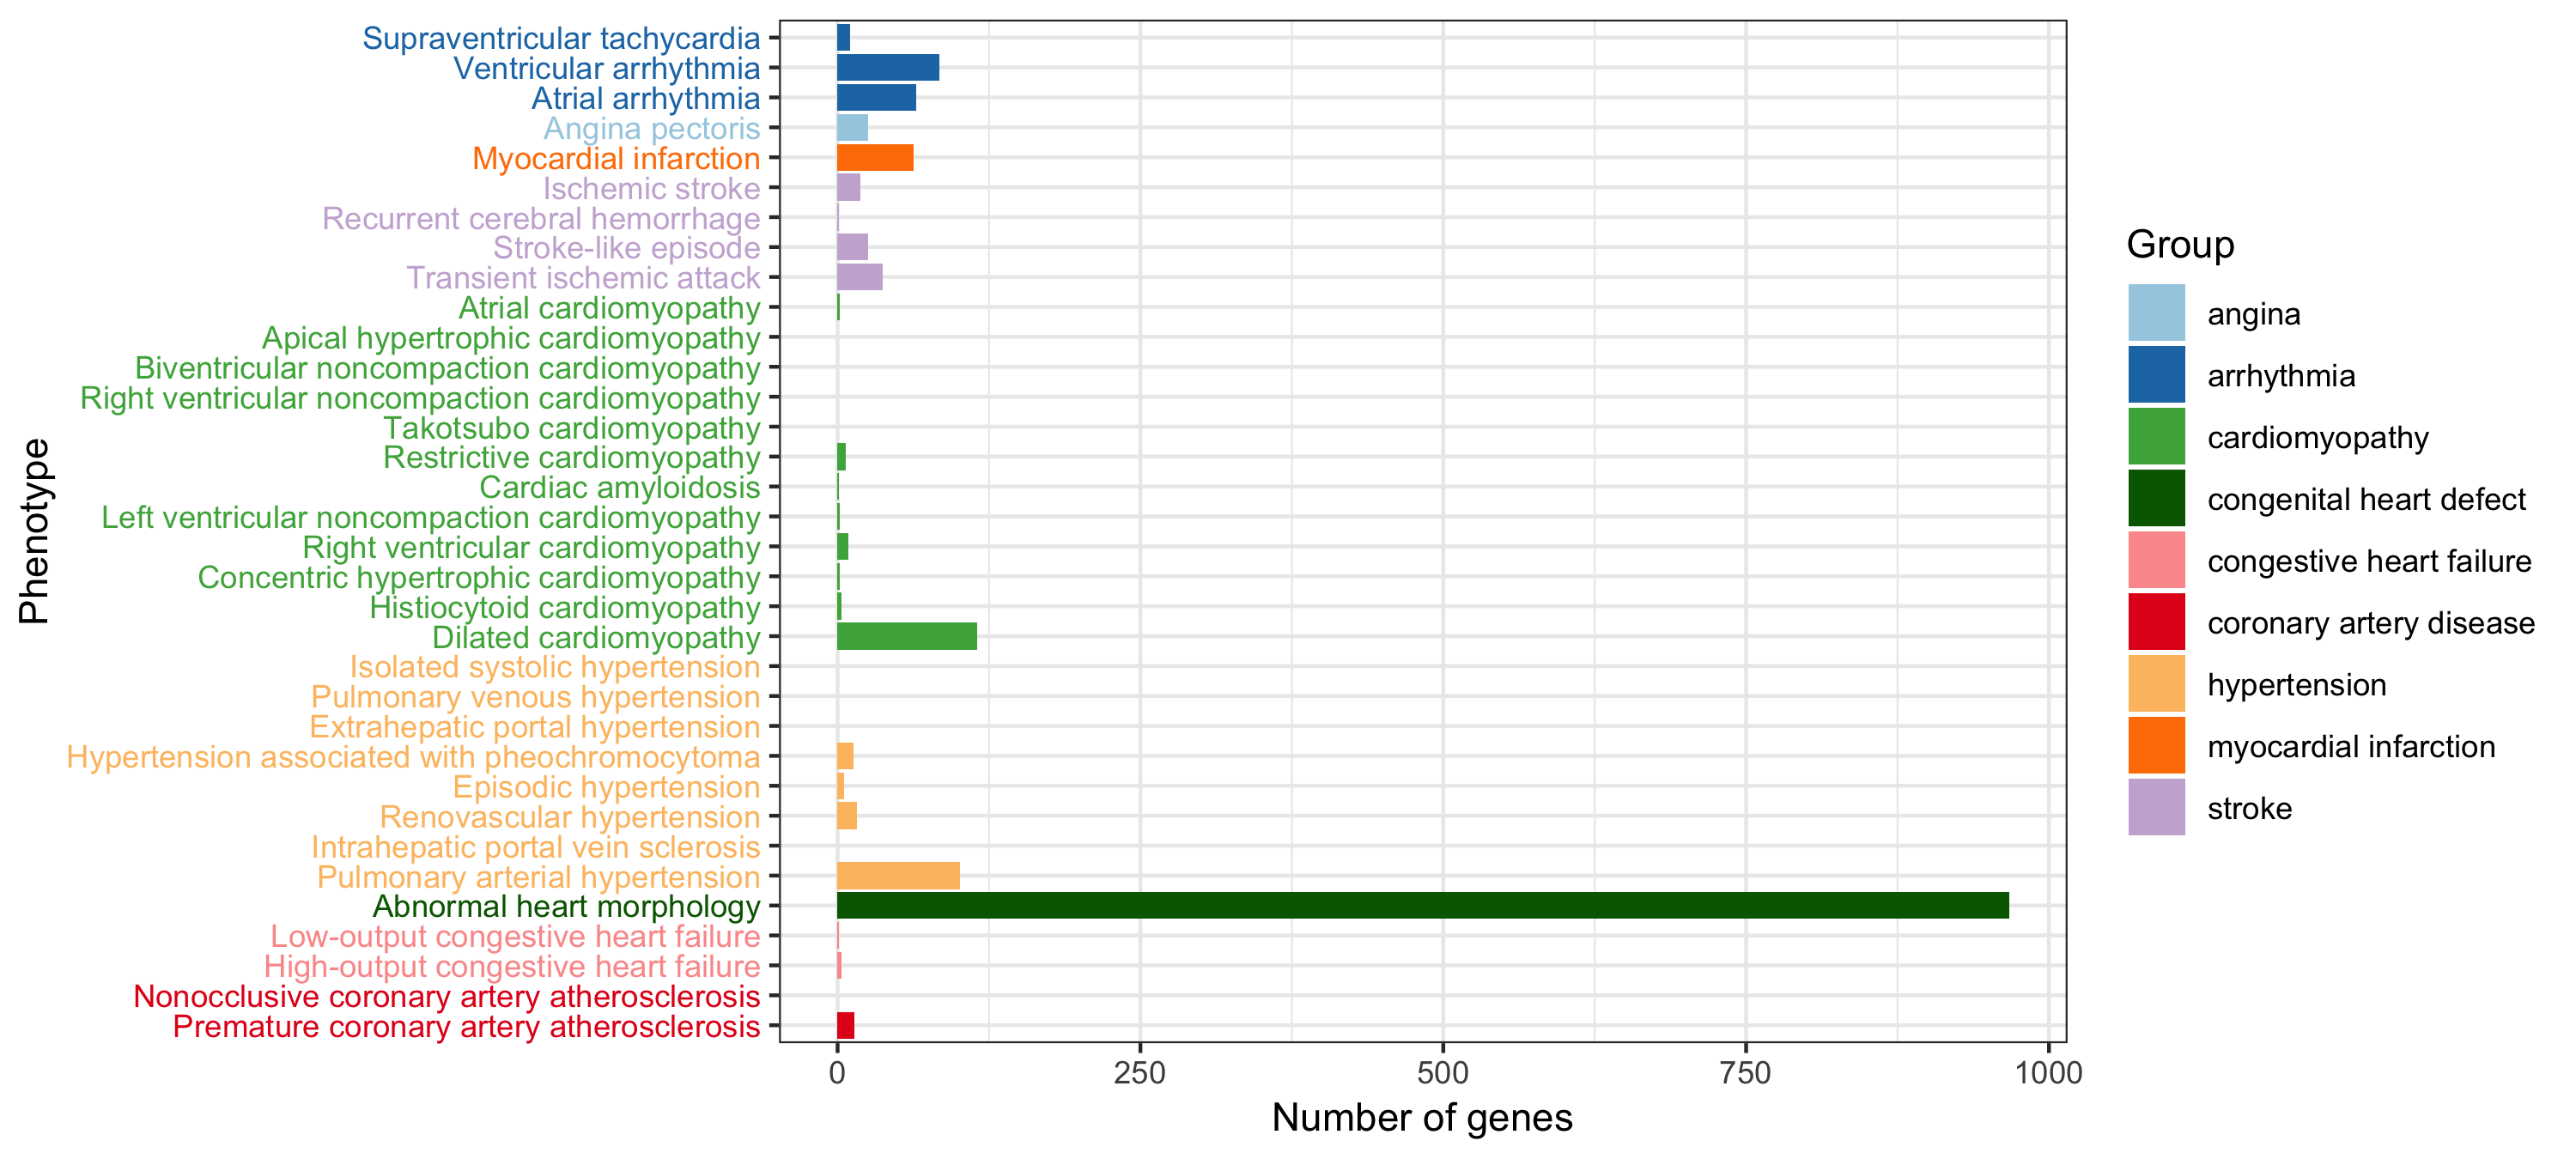
\includegraphics[width=1.\linewidth]{hpo-gene-count}
	\caption{The number of genes associated with \textit{Abnormality of the cardiovascular system} (HP:0001626) as reported in the Human Phenotype Ontology \citep{Kohler:2014:Human}, with phenotype annotations pooled from OMIM, ORPHA and DECIPHER.}
	\label{fig:hpo_gene_count}	
\end{figure*}


\subsection{The diversity of actors}

Our understanding of CVD has been critically limited by the technical capability in characterizing various molecular fractions of a cell. GWA studies are predominantly conducted on SNPs thanks to the availability of easy-to-produce SNP microarrays. Such technologies have clearly enriched our knowledge base of single nucleotide variants, while leaving structural variations poorly understood. There are now 660 million of SNPs documented in dbSNP, compared to 4.6 millions of structural variations in the DGVa (Database of Genomic Variants Archive, which also includes studies annotated by the NCBI-hosted database of structural variants dbVar) \comment{number from Ensembl, but is it really this much?}. Although structural variation databases are still primordial form of study archives, rather than data entries for structural variations, the map of SV from 1000 Genomes Project \citep{Sudmant:2015:integrated} has enabled further studies of the role of SV in cardiac diseases, suggesting at least the impact of SV on the transcriptional regulation of cardiac genes expressed in the heart \citep{Haas:2018:Genomic}. As envisioned, structural variations might be one of the promising lands to look for the missing heritability in CVD \citep{Eichler:2010:Missing}.

%Reliable identification of structural variants is an open challenge being addressed by more research recently. Cardiovascular disease offer a concrete and narrow space to facilitate the exploration of this area.

% non-coding
When array-based genotyping was gradually replaced by next-generation sequencing, the cost of sequencing an \textit{exome}, the protein-coding part of a genome, became much more affordable and enabled the collection of more than 60000 exomes \citep{Lek:2016:Analysis}. Using this data set, \cite{Walsh:2017:Reassessment} have found that many genetic variants associated with various cardiomyopathy diseases turned out to be equally common in clinical cases as in the control population, showing that . Sample size this large has been looking forward to for studying of rare variants. It turned out allowed rare variants to be observed with more power, leading to a somewhat surprising observation about many rare variations in cardiomyopathy diseases.

, the sequencing of exome, defined as the protein-coding part of the genome, was prioritized over that of the whole genome, based on a regularly cited fact that exome harbors 85\% of the disease-causing variants \citep{Antonarakis:2001:nature}. This figure turns out to be an outdated estimate from 1995. Our survey of all associations in the GWAS catalog \citep{MacArthur:2017:new} ( manually curated to retain only those with p-value less than $10^{-5}$) revealed that a large fraction of variants occur in non-protein coding regions such as intronic, intergenic, and splice junctions (Figure \ref{fig:variant_context}). Interestingly, the distribution of CVD-associated variants mimics that of the all-variant set, suggesting that variants accounting for human traits, neutral or disease-causing, might be distributed in the same manner across the genome.

With




%epigenetics

Epigenetics, by definition, includes all the heritable modifications that occur without the changes in DNA sequences. Epigenetic processes involve DNA methylation, histone modifications, and the less well-defined group of non-coding RNAs.


Thanks to the advance of next-generation sequencing techniques, the prevalence of long non-coding RNAs in cardiovascular diseases has emerged. A range of functions have been reported for lncRNAs, including imprinting, scaffolding, enhancer, and molecular sponges. More research is certainly needed to obtain a complete catalog of lncRNA functions. \comment{role of non-coding RNAs and epigenetics in cardiovascular biology \citep{Sallam:2018:Long}}

chromatin conformation \citep{Rosa-Garrido:2017:HighResolution}




environment interactions

A critical limitation to study at the molecular level is the interaction between gene  and environment.

It has been known for decades that non-genetic factors play a critical role in cardiovascular health, such that a risk prediction using lifestyle variables perform much better than a gene-count score \citep{Joyner:2011:Ten}. The understanding of this interaction at the molecular level is still relevant for basic research, as well as health care applications. The research has been limited due to the difficulties in monitoring one's external environment. Such barrriers start to be lifted, thanks to the development of wearable devices that can collect real time data in a non-intrusive manner. Studies on the exposome have started to accumulate \citep{Jiang:2018:Dynamic}, projecting the greater need of large scale, streaming data analysis.


\subsection{The forgotten concepts}

homeostasis

omnigenic model remind us about the widespread interactions possible in a cell and how important it is to account for most of the actors

%Accordingly, the number of biological states is exponential. Among these states, it is obvious that biological systems do not seek for a single optimal state, but always strive for the most convenient functional one. Therefore, it is reasonable to expect a diverse set of states in which biological system is equivalently functional.



\begin{figure}[!tpb]
	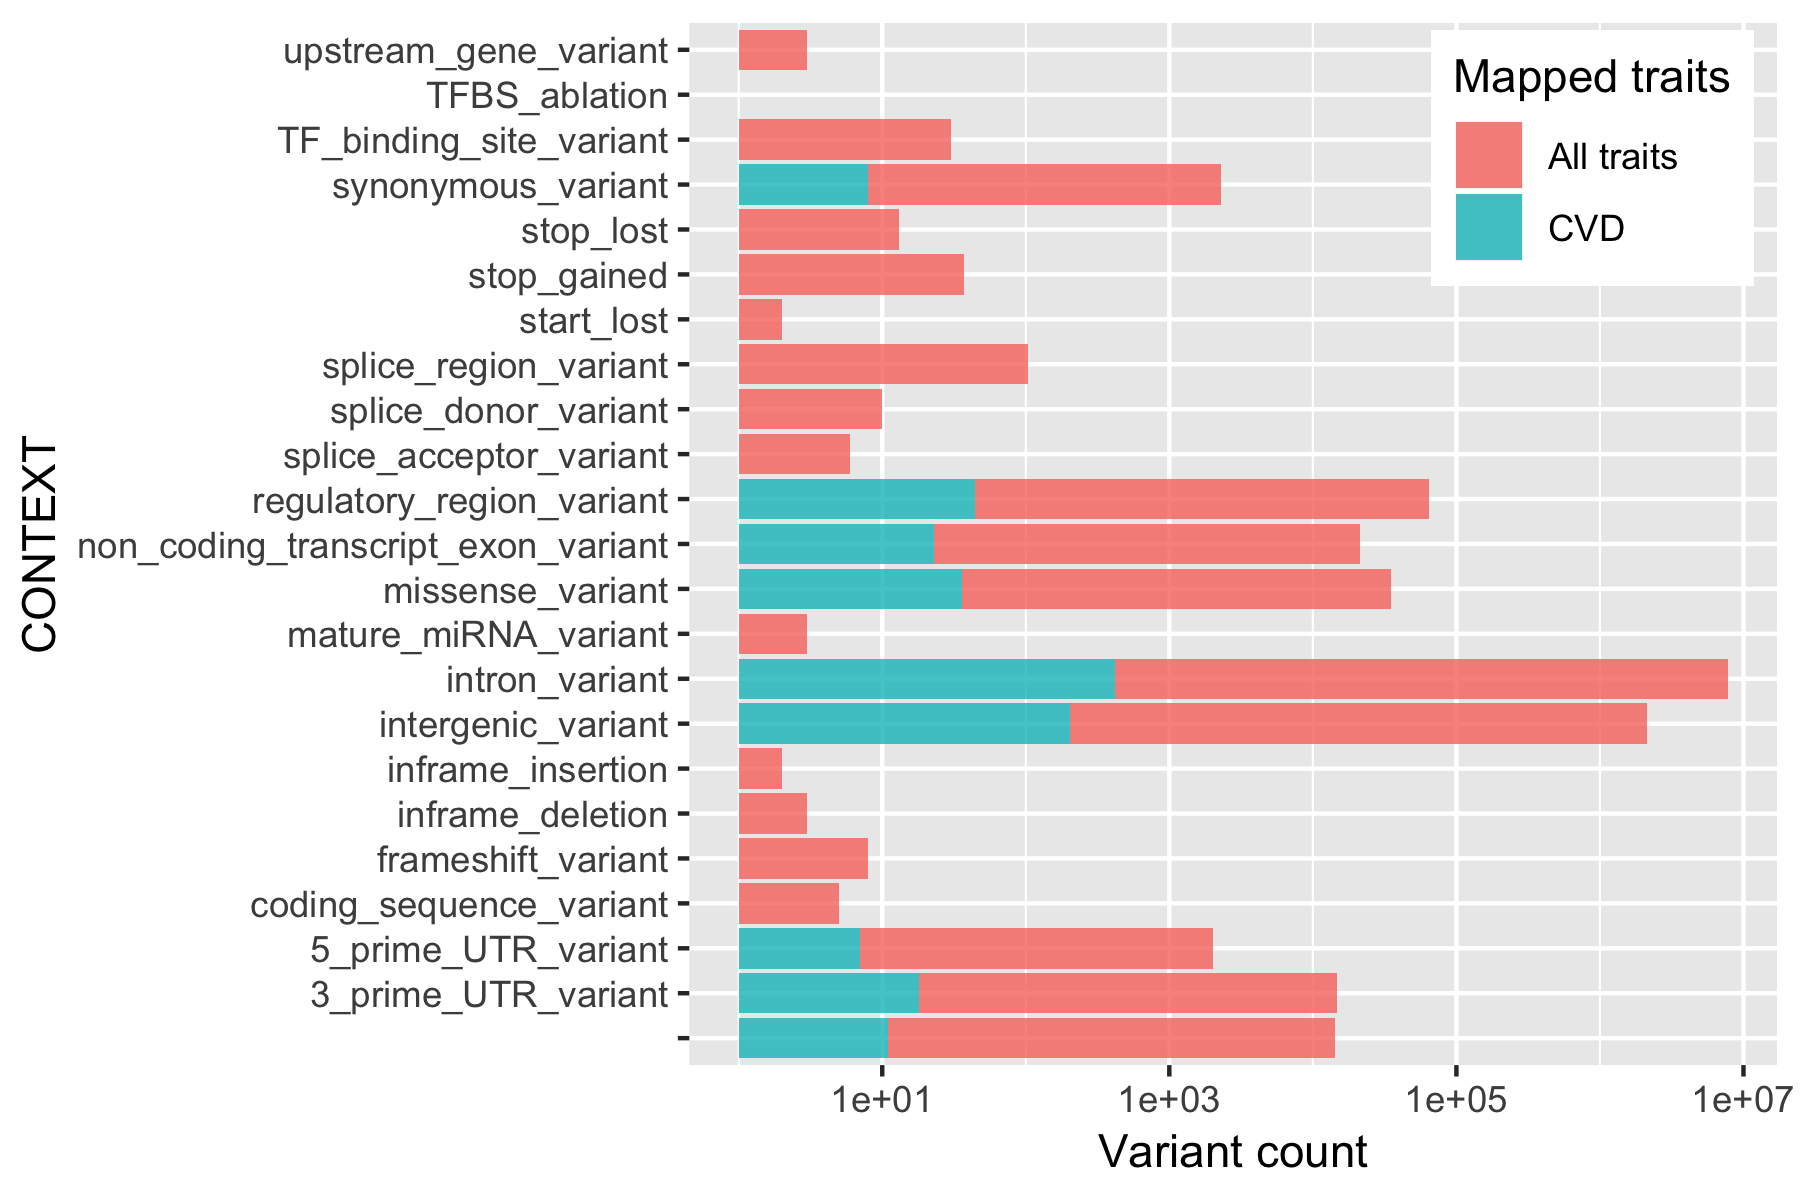
\includegraphics[width=1\linewidth]{variant_contexts_sigVars}
	\caption{Distribution of known variants in the human genome. \comment{Trang: group the contexts into 4 catergories: intronic, splice, intergenic and exonic regions, either by colors or additional chart.}}
	\label{fig:variant_context}
\end{figure}

%Some quantity showing the associations of CVD with genes...
%




%
\section{Cardioinformatics}
%%
As demonstrated earlier, the large number of studies have contributed to a larger, not necessarily more solid, body of knowledge. In the following section, we argue for the readiness and the prospect of cardioinformatics, by looking at the current infrastructure for biological data analytics, the computational methods.

\subsection{The soil is worked}

This part is to introduce the achievements and on-going work in developing the infrastructure for data storage, management and sharing, thus making the case for an invest in bioinformatics analyses to capitalize on these resources.


\subsubsection{Profusion of data}


This part is to demonstrate the volume of existing data and the potential of new insights from re-analyses, especially when more than one layers are stacked. Give the examples of those multi-omics studies.


\comment{Tentative: A figure/table enlisting layers of modifications that contribute to determine a phenotype, with the corresponding experimental techniques}

\cite{Santolini:2018:personalized} 

\cite{Klarin:2017:Genetic}

Technological advances brought about the accumulation of biological data, both in the number of data points, and the number of dimensions in each data point.
High-throughput profiling techniques are inarguably the main drive in creating high-dimensional data (DNA, RNA, protein levels).
A glimpse into central repositories such as GEO or dbGaP hinted at the amount of data points that can be accumulated from small  studies. Depending on the questions at hands, the precise definition of a data point can vary. In most cases, it can be equivalent to the number biological samples or that of individual donors. Although studies directly related to CVDs are of interest when it comes to future CVD research, a significant number of data points from non-CVD studies can be put into use, for example, when these studies investigated samples of cardiovascular origin (heart or vascular tissues).

\begin{figure}[!tpb]%figure1
	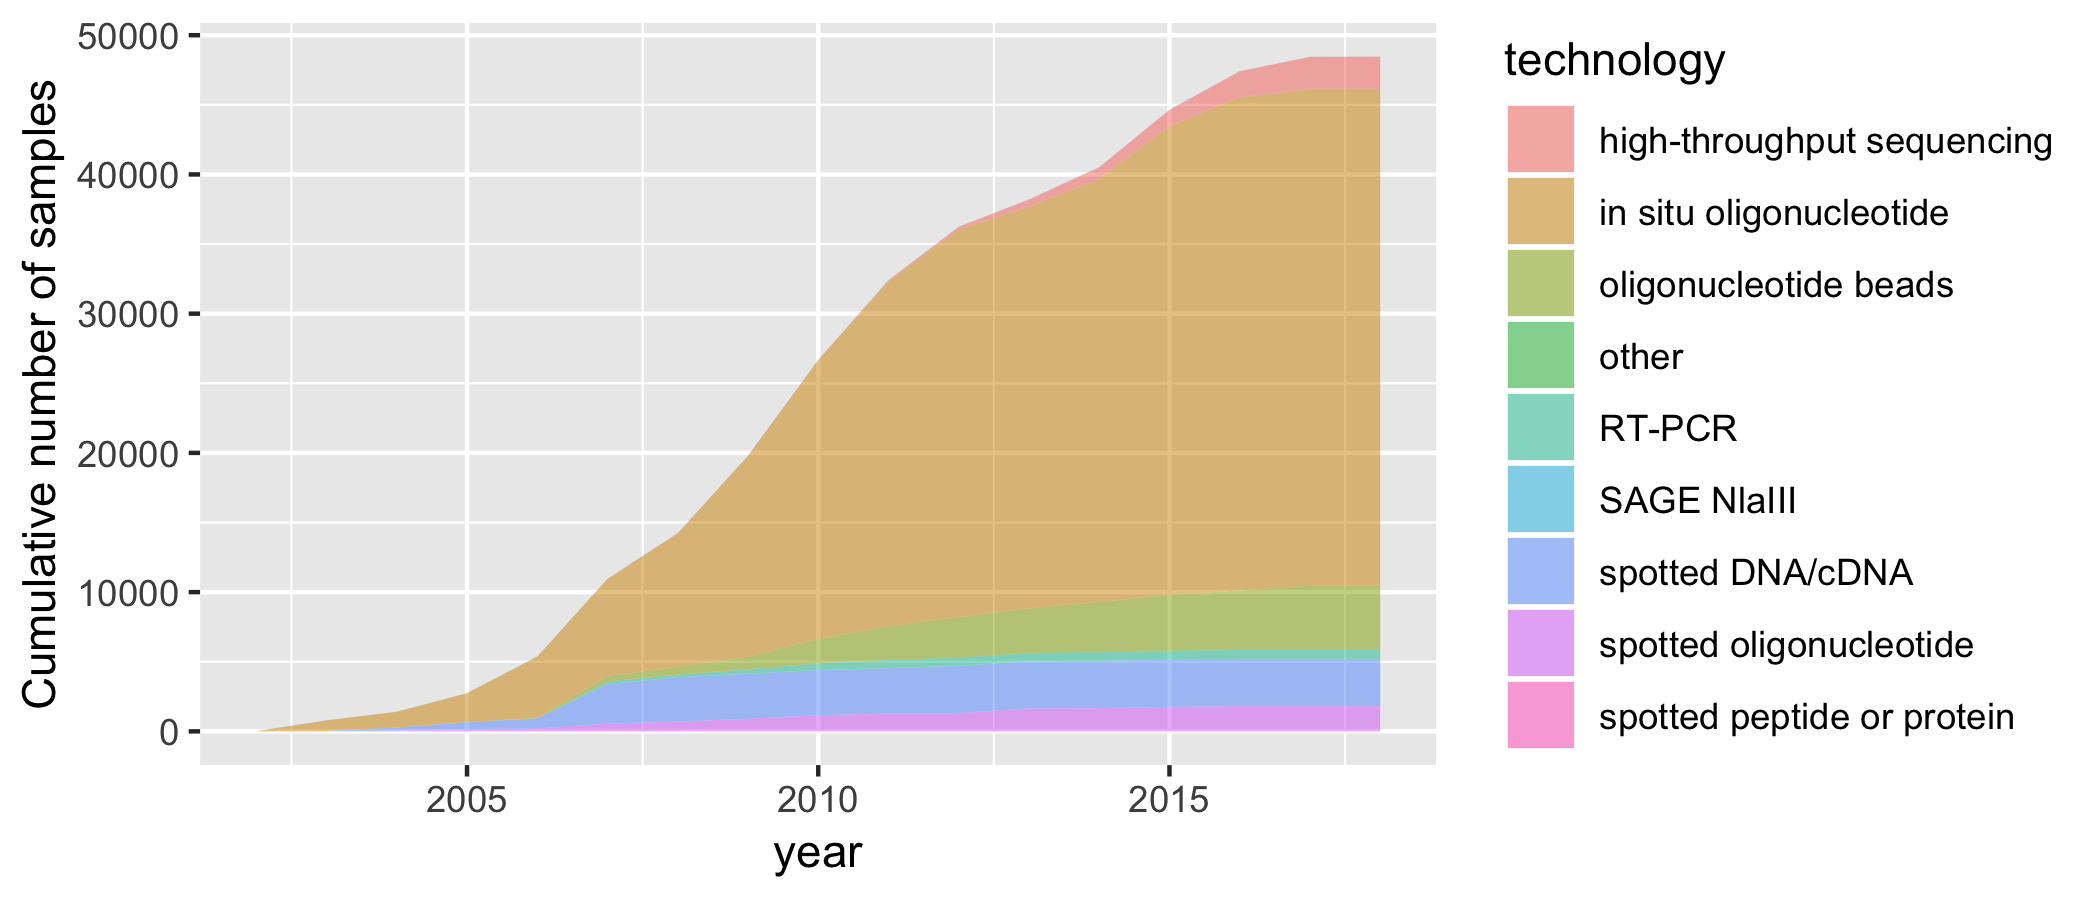
\includegraphics[width=1\linewidth]{gsm_count_by_tech.png}
	\caption{The cumulative number of samples deposited on GEO.}
	\label{fig:01}
\end{figure}

\begin{table}[!t]
	\processtable{Number of samples available on GEO that are of potential use of cardioinformatics research, including those deposited by CVD studies and non-CVD studies.\label{tab:geoSamples}} {\begin{tabular}{@{}llll@{}}\toprule 
			molecule &non-CVD studies & CVD studies \\ \midrule
			genomic DNA &            440 &        8525  \\
			polyA RNA &             89 &         392  \\
			total RNA &           2974 &       39540  \\
			other &             NA &           5  \\
			protein &             NA &           3  \\ \botrule
	\end{tabular}}{This is a footnote}
\end{table}

The figures given in Table \ref{tab:dbgapSubject} are in fact the conservative estimates of the data generated so far among the research community. A much larger amount of data are stored on dbGaP and accessible upon approval of data request. Among these, the number of subjects involved in CVD research alone are more than 600000. %658305 to be exact
In term of subject count, the amount of data from CVD-related studies permitted for General Research Use is only
% 16786 / 658305
2.5\% of all the CVD-related studies deposited on dbGaP.

\todo{supplement table if necessary}

Aside from central authoritative repositories of research data, smaller databases with narrower focus are budding. For example, many databases have been created to collect chromatin structure data from 3C, 4C, 5C and HiC-seq experiments. A few databases are actively gathering knowledge about non-coding RNAs. Being in these under-explored territories, researchers may need more work to collect and curate their data from multiple sources before using them for further analyses.

A number of projects have successfully re-processed and re-analyzed the large amount of biological samples across large databases such as TCGA, dbGaP, etc., providing novel insights or cloud-compatible analytics protocols (Rail-dbGaP \citep{Nellore:2016:RaildbGaP}, Toil \citep{Vivian:2017:Toil}). These successes on one hand demonstrate the great potential of existing data sets, and on the other, provide concrete examples on how cloud-based computing can be performed, to overcome huge requirements of storage, memory and computational power. More than 20 providers are actively provisioning cloud services in both commercial and academic sectors \citep{Langmead:2018:Cloud}, promising even lower cost and higher accessibility.

A list of databases focusing on human genotype-phenotype data was already presented elsewhere \citep{Brookes:2015:Human}, illustrating the expansion of data available to biomedical research. The figures in Table \ref{tab:dbgapSubject} exemplify a prominent issue in making these data more accessible. A promising solution, the DataSHIELD platform to enable sensitive data analytics without physical nor direct access to the data \citep{Gaye:2014:DataSHIELD}, has been available for years and is now enabling wider applications \citep{Wilson:2017:DataSHIELD}.

One common way to access genotype-phenotype data is to file a request, prepare the computing facility, implement the security measures, and transfer the data upon approval. This mode of access is currently applied for all control-accessed data in dbGaP, adding a significant administrative burden to researchers who need access to the data. The AHA Precision Medicine Platform \citep{Kass-Hout:2018:American} has simplified this process significantly by streamlining the search, request and transfer of data to be analyzed on a secured cloud-based workspace.


% Please add the following required packages to your document preamble:
% \usepackage{booktabs}
\begin{table}[]
	\caption{The subject count aggregated from studies deposited in dbGaP, licensed for General Research Use}
	\label{tab:dbgapSubject}
	\begin{tabular}{l l l}
		\toprule
		& \textbf{CVD} &  \textbf{All}                         \\ \midrule
		16s rRNA (NGS)                 &     0 &      92 \\
		CNV Genotypes                  &     0 &   48972 \\
		Chromatin (NGS)                &     0 &     139 \\
		Genomic Sequence Amplicon (NGS)&     0 &       8 \\
		Methylation (CpG)              &     0 &     657 \\
		Methylome sequencing           &     0 &     152 \\
		QTL Results                    &     0 &     281 \\
		RNA Seq (NGS)                  &   333 &    1498 \\
		SNP Genotypes (Array)          &  6658 &  113597 \\
		SNP Genotypes (NGS)            &  4277 &   11786 \\
		SNP Genotypes (PCR)            &     0 &      10 \\
		SNP Genotypes (imputed)        &     0 &   29693 \\
		SNP/CNV Genotypes (NGS)        &     0 &     936 \\
		SNP/CNV Genotypes (imputed)    &     0 &    9291 \\
		SNV (.MAF)                     &     0 &       2 \\
		SNV Aggregate (.MAF)           &     0 &     570 \\
		Targeted Genome (NGS)          &     0 &    9918 \\
		Whole Exome (NGS)              &  5518 &   12771 \\
		Whole Genome (NGS)             &     0 &    1245 \\
		mRNA Expression (Array)        &     0 &     798 \\
		miRNA (NGS)                        & 0 &   228 \\ \hline
		Total subject count & 16786 & 242644 \\ 
	\end{tabular}
\end{table}


\subsubsection{Infrastructure}

The infrastructure for bioinformatics analyses now is even more mature, thanks to cloud computing \citep{Langmead:2018:Cloud}, secured data storage and management.

Guidelines, protocol


Data visibility


efforts to standardize data management and sharing

%
%\subsubsection{Basic research}
%for data management, computational analysis, visual representation, etc.
%
%\subsubsection{Clinical application}
%
%

\subsection{Computational methods}


As early as 1999 when the complete human genome and high-throughput transcriptomic profiling are on the horizon, research community have started to recognize the critical use of bioinformatics analyses in generating insights from these data. The computational approaches outlined by \cite{Claverie:1999:Computational} for the early day gene expression data are still popular in today transcriptomics studies: differential gene expression analysis, co-expression analysis and gene clustering with subsequent identification of enriched biological pathways. Those old-fashioned methods can still bring fruitful analyses, as illustrated in a recent study on heart failure \citep{Santolini:2018:personalized}. A significant improvement in the power of differential expression analysis is the large number of samples which will be highly difficult to obtained in individual studies. Opportunity: re-analysis of newly compiled data, framework to enable streaming analysis as new data is deposited.


The combination of different layers of omics data is the most useful when they are collected simultaneously. However, even when they are not collected for the same samples, the additional layers can still be of great value, for example, to serve as priors. Examples

* proteomics + transcriptomics \citep{Uhlen:2015:Tissuebased}
* genomics + transcriptomics \citep{Klarin:2017:Genetic}



The application of machine learning will be indispensable in many aspects of cardiology \citep{Shameer:2017:Translational,Shameer:2018:Machine}. Given the availability of machine learning performant implementations, cardioinformatics is better positioned to tackle domain-specific questions and develop clinical application. For example, ML can be applied to enhance medical image. In basic research, natural language processing can be a promising tool to improve data collection and organization.

With less focus on computation, visualization still makes up an important part in facilitating biological research, especially for data exploration, pattern recognition, and data representation. Visualization methods are blooming to accommodate the diverse data types in biology \citep{Pavlopoulos:2015:Visualizing}. With regard to visualization, the exciting challenge to cardioinformatics researcher is the meaningful integrated representation of data layers. In basic research, such representation can mean to put together pieces of information from various experimental techniques. In clinical application, the focus is on facilitating clinical decisions.

Visualization of chromatin 3D structure emerges as a demand to analyze and present experimental data from conformation capture experiments. The challenges posed by these experiments, being new, high-throughput and  3-dimensional, are actively researched visualization problems \citep{Goodstadt:2017:Challenges}. As a researcher in cardiovascular disease, it is important to stay abreast with the developments in this field to make the most use of the available data.

Search engine and knowledge synthesis \citep{Lutjohann:2011:Sciencenet}. A universal element of all research, knowledge synthesis is under-rated research task. Like most other areas, most of the work in knowledge synthesis has been and has to be done manually in cardiovascular research. Cardiovascular diseases impose the challenge of understanding complex systems of multiple dimensions, creating the pressing need of summarizing and synthesizing knowledge from the vast body of research in a more robust manner. Natural language processing.


The bottleneck in the application of these computational methods are not in their implementation, but in the shortage of domain knowledge. Many generic bio-portals have been published in the recent years, aiming to make complicated data as accessible as possible to a general audience. The lack of focus on a research topic has limited their usefulness. Cardioinformatics, as 
%\subsection{The multi-layered paths from genome to phenotype}


%%
%\begin{itemize}
%	\item genome
%	\item epigenome
%	\item transcriptome: mRNA, non-coding RNA: microRNA, long non-coding RNA
%	\item 	proteome
%	\item	metabolome
%\end{itemize}
%%environmental factors
%
%

\subsection{New and re-newed perspectives}

Cardioinformatics offers a number of powerful concepts to investigate complex physiological system.

The paradigm shift from the physical genes to the "eigengenes" in studying complex diseases \citep{Weiss:2012:Good} is a pragmatic approach. This approach allows one to focus on mimicking the healthy system without the knowledge required to model the individual actors and their interactions, making it an ideal method in the drug discovery workflow. The paradigm can help advancing knowledge further because it suggests an efficient way to engineer biological system and learn how it works.

The heavily connected biological system is among many types that can be modeled and analyzed as graphs. The omnigenic model recently proposed has highlighted the need for this system-level modeling, since the involvement of peripheral genes are widespread in physiological and pathological processes.

\subsection{Prospective development}



\section{Conclusion}


%

\enlargethispage{12pt}




\section*{Acknowledgements}

Text Text Text Text Text Text  Text Text.  
\vspace*{-12pt}

\section*{Funding}

This work has been supported by the... Text Text  Text Text.\vspace*{-12pt}

\bibliographystyle{natbib}
%\bibliographystyle{achemnat}
%\bibliographystyle{plainnat}
%\bibliographystyle{abbrv}
%
%\bibliographystyle{plain}
%
\bibliography{cardio}



\end{document}
